%!TEX root = main.tex

\section{Decreasing Reward}
\label{sec-dec}

%While interesting, readers could argue that the payoff function considered before is not completely modelling bitcoin, because in bitcoin 
%the reward given for mining blocks is reduced by half every 200.000 blocks or so. Thus the natural question, do the results above continue to hold under these 
%circumstances? Our answer is a resounding no, and now forking can be a valid strategy depending on the hash power of a player (and the other parameters of the game). 

Miner's fees in many cryptocurrencies, including Bitcoin, is not constant, but diminishes over time~\cite{Bitcoin,Monero,Litecoin,Bcash}. We model such 
%diminishing 
fees as a constant factor that is lowered after every new block in the blockchain. That is, 
%in this section 
we use the following reward function $\rpa$ for all players $p \in \bP$, denoted as the \textbf{$\alpha$-discounted reward}: 
%\begin{eqnarray*}
%\rpa(q) & = & 
%{\displaystyle c \cdot \sum_{i=1}^{|\meet(q)|} \alpha^i \cdot \chi_p(\meet(q),i)} \end{eqnarray*}
\begin{eqnarray*}
\rpa(q) & = & 
c \cdot \sum_{b \in \meet(q)} \alpha^{|b|} \cdot \chi_p(b),
\end{eqnarray*}
In this section, we show that when miners' fees decrease over time, doing a fork can be a good strategy. In fact, we explore in Sections~\ref{sec-forkingstrategies} and \ref{sec-giving-up} several strategies based on the maximum length of the fight the miner is willing to carry out when doing a fork, and how far back the miner is willing to do a fork. Interestingly, for such strategies we confirm the folklore fact that it is profitable to fork with more than half of the hash power. Moreover, our exploration in Section \ref{sec-giving-up} gives us a concrete strategy that with less than half of the hash power 
%a little more than $46\%$ of the hash power 
can be used to defeat the default strategy.

%Thus, it is natural to ask whether mining on top of the existing blockchain continues to be an optimal strategy under these 
%circumstances. 
%%Our answer is a resounding no, and as we show in this section, when the miner fees decrease over time, forking can be a valid strategy depending on the hash power of the player (and other parameters of the game).
%As shown in this section, the answer to this question is no; when the miner's fees decreases forking can be a good strategy, depending on the hash power of a player and on the other parameters of the game.
%
%For simplicity, we model the diminishing miner's fees as a constant factor that is lowered after every new block in the blockchain. That is, in this section 
%we use the following reward function $\rpa$ for all players $p \in \bP$, denoted as the \textbf{$\alpha$-discounted reward}: 
%%\begin{eqnarray*}
%%\rpa(q) & = & 
%%{\displaystyle c \cdot \sum_{i=1}^{|\meet(q)|} \alpha^i \cdot \chi_p(\meet(q),i)} \end{eqnarray*}
%\begin{eqnarray*}
%\rpa(q) & = & 
%c \cdot \sum_{b \in \meet(q)} \alpha^{|b|} \cdot \chi_p(b),
%\end{eqnarray*}
%where $c$ is a positive real number and $\alpha \in (0,1]$. Notice that in the case of Bitcoin, $\alpha$ has to make the reward halve every 210.000 blocks, and is therefore very close to 1. %This is usually the case in other cryptocurrencies as well. 
%
%%\medskip
%%
%%(say that the approach we use is the same as above: we consider a two player game and group a bunch of well behaved players 
%%into a single player. Also state that the subtree lemma holds also for this payoff)

\subsection{When doing a fork is a good strategy?}
\label{sec-forkingstrategies}

To calculate when doing a fork is a viable option, we consider a scenario when one of our $m$ players decides to deviate from the default strategy, while the remaining players all follow the default strategy. 
%This is similar the question a miner with a lot of hash power is likely to ask, since she would like to determine whether it suites her to try and force a fork in order to own more blocks in the new blockchain. 
The first observation is that in this case we can reduce the $m$ player game to a two player game, where all the players following the default strategy are represented by a single player behaving as the protocol dictates, with the combined hash power of all these players. Therefore in this section we will consider that the mining game is played by two players 0 and 1, where 0 represents the miners behaving according to the default strategy, and 1 the miner trying to determine whether doing a fork is economically more viable than mining on the existing blockchain. We always assume that the player 1 has hash power $h$, while player 0 has hash power $1-h$.

In order to determine whether there is an incentive for player~1 to do a fork, we first need to determine her utility when she is playing according to the default strategy $\cdf = (\df_0,\df_1)$. 

\begin{lemma}\label{lem:default_utility}
If $h$ is the hash power of player 1, then:
%and the strategy deployed by the two players is $\cdf$, then the utility of player 1 is given by the expression:
\begin{eqnarray*}
u_1(\cdf) & = & h\cdot c\cdot\frac{\alpha\cdot\beta}{(1-\alpha\cdot\beta)}.
\end{eqnarray*}
\end{lemma}
As in the case of constant reward, this corresponds to $h$ times the utility of winning all the blocks in the single blockchain generated by the default strategy.

%In this section, players $\{0,1\}$ play according to the default strategy, defined in section \ref{sec-defstrategy}. For any state $q$ of the game, $\mathcal{T}(q)$ consists of a single branch and therefore \bchain$(q)$ is always defined. Moreover, given the behavior of players we can write $q$ uniquely as a binary sequence $w\in\{0,1\}^{\mid q\mid }$ encoding the chronological history of the game until $q$ is reached, where $p\in\{0,1\}$ stands for ``player $p$ appends a block''. In other words, there are bijections $ \bQ \simeq\bchain(\bQ)\simeq \{0,1\}^\ast$. This encoding proves useful as we have
%\begin{eqnarray*}
%	r_p(w) &=&	c\cdot \sum_{j=1}^{\mid w\mid}w[j] \alpha^j \\
%	\pr^{\df}(w \mid \varepsilon) &=&	h^{H(w)}(1-h)^{|w|-H(w)}
%\end{eqnarray*}
%where $H(x)$ denotes the Hamming weight of integer $x$, defined as the amount of non-zero bits of $x$. We prove the following.

Now suppose that player $1$ deviates from the default strategy, and considers a strategy based on forking the blockchain once player $0$ mines a block. 
How would this new strategy look? To consider a realistic scenario, in this section we 
%study the following strategies. 
%
%Juan: this is better as a comment once we analyse stuff
%For simplicity we only consider the situation where both players $0$ and $1$ begin the game in the genesis block, but this is without generality: 
%any state before player $1$ deviates is just a sequence of blocks, a blockchain, and thus we can always sum up any reward player $0$ or $1$ is collecting thanks to the blocks in this 
%sequences. 
%
%\begin{itemize}
%\item 
%First we 
consider the strategy $\af$ (for \emph{always fork}), where player~$1$ forks as soon as player $0$ mines a block in the blockchain, and she continues mining on the new branch until it becomes the blockchain. Here player $1$ is willing to fork every time player $0$ produces a block in the blockchain. In other words, 
in $\af$, player~$1$ tries to have all the blocks in the blockchain. This strategy is depicted in Figure~\ref{fig:always_fork}.
%\item 
%Second, we consider a family of strategies $\pf{1}$, $\pf{2}$, etc. In the strategy $\pf{i}$, player $1$ behaves just as in $\af$, but will do a fork at most $i$ times, %a specific number of times, 
%switching to $\df$ once 
%all these forks have been completed. Coming back to Figure \ref{fig:always_fork}, if player $1$ plays according to $\pf{1}$ instead of $\af$, then she would fork upon block $0$, but 
%would continue mining on block $1110$ instead of forking again. 
%\end{itemize}

\begin{figure}
\begin{center}
\begin{tikzpicture}[->,>=stealth',auto,thick, scale = 0.6,state/.style={circle,inner sep=2pt}]

    % The graph
	\node [state] at (-0.2,0) (R) {$\varepsilon$};
	\node [state] at (1.5,0.70) (1) {$1$};
	\node [state] at (1.5,-0.70) (0) {$0$};

	\node [state] at (3.3,0.70) (11) {$11$};		
	\node [state] at (5.2,0.70) (111) {$111$};
	\node [state] at (7.4,0.70) (1110) {$1110$};

	\node [state] at (7.4,1.80) (1111) {$1111$};
	\node [state] at (9.8,1.80) (11111) {$11111$};
	
	%\node [state] at (4.6,1.5) (111) {$111$};
	%\node [state] at (6.2,1.5) (1111) {$1111$};

	% Graph edges
	\path[->]
	(R) edge (0)
	(1) edge (11)
	(11) edge (111)	
	(111) edge (1110)
	(1111) edge (11111);
	
	\path[->,dashed]
	(R) edge (1)
	(111) edge (1111);
	
%	(11) edge (111)
%	(111) edge (1111);

\end{tikzpicture} 
\end{center}
%\caption{Dashed arrows are used to indicate when player~1 did a fork. Initially, player $0$ mines on the genesis block $\varepsilon$ including block $0$. Player 1 then decides to fork on the genesis block, and continue mining in this new brach until it becomes the blockchain, which happens in this case when player 1 mines on top of block $1$ generating block $11$. But then again player 1 loses a block when player 0 mines on top of block $111$ generating block $1110$, so she decides to fork on top of block $111$ until the new brach becomes the blockchain. Up to this point in the mining game, the blockchain is given by the path $\{\varepsilon, 1, 11, 111, 1111, 11111\}$ that only contains blocks belonging to player 1.}
\caption{Dashed arrows are used to indicate when player~1 does a fork. The first block (block 0) is mined by player 0. At this point, player 1 decides to fork (mining the block 1), and successfully mines the blocks 11 and 111 on this branch. When player 0 mines the block 1110, player 1 decides to fork again, mining the blocks 1111 and 11111.}
%
%until the new brach becomes the blockchain
%which is represented by a dashed arrow, after she manages to Player Following the block 0 player 1 tries to win a fork starting at $\varepsilon$. After winning the initial fork, if she loses another block (as in the block 110), she will try to fork again. When playing $\baf$, the word $w$ describing this state is $011011$.}
\label{fig:always_fork}
\end{figure}

%\medskip
%\noindent
%\textbf{Strategy $\af$}. 
\subsubsection{The utility of always forking}
%As we explained, the idea of $\af$ for player $1$ is to fork every time she loses a block, trying to own all blocks in the blockchain. 
The question we want to answer is twofold. On the one hand, we want to know whether $\af$ is a better strategy than $\df_1$ for player $1$, under the assumption that player $0$ uses $\df_0$, and under some specific values of $\alpha$, $\beta$ and $h$. 
%Since we know how to compute the utility for $\bdf = (\df_0,\df_1)$, this amounts to computing the utility for player $1$ for the combined strategy $(\df_0,\af)$. 
On the other hand, and 
perhaps more interestingly, we can also answer a more analytical question: given realistic values of $\alpha$ and $\beta$, how much hash power does player $1$ need to consider $\af$ instead of $\df_1$? 
Answering both questions requires us to compute the utility for the strategy $\baf=(\df_0,\af)$, which is what we do next. 

\begin{theorem}\label{thm:always_fork}
If $h$ is the hash power of player 1, then:
%%, $\baf=(\df_0,\af)$ be the strategy deployed in the mining game, and let $Cat$ be the generating function of Catalan numbers. Then:
\begin{eqnarray*}
u_1(\baf) &=& \frac{\Phi}{1-\Gamma}, \mbox{ where}
\end{eqnarray*}
%{\small
\begin{align*}
\Phi & \ = \ \frac{\alpha \cdot \beta \cdot h \cdot c}{(1-\alpha)} \cdot \big[\cat(\beta^2 \cdot h \cdot (1-h)) - \alpha\cdot \cat(\alpha \cdot \beta^2 \cdot h \cdot (1-h))\big],\\
%& \hspace{100pt} \alpha\cdot \cat(\alpha \cdot \beta^2 \cdot h \cdot (1-h))\big),\\
\Gamma & \ = \ \alpha \cdot \beta \cdot h \cdot \cat(\alpha\cdot \beta^2 \cdot h \cdot (1-h)),
\end{align*}
%}
and $\cat(x) = \frac{1-\sqrt{1-4x}}{2x}$ is the generating function of Catalan numbers.
\end{theorem}

%ADD FORK ONCE

%Of course, if player 1 knows that her utility will be higher when she forks in the genesis block as opposed to playing the default strategy, then why not repeat the fork every time she loses a block? After all, if she is likely to win one fork, she is likely to win multiple forks as well. Let $F_\infty$ be a strategy for player 1 where she tries to have all the blocks in the blockchain. That is, in $\af$, player one will fork every time she loses a single block. This strategy is depicted in Figure \ref{fig:always_fork}. We can now obtain the following.

Before presenting the proof of Theorem \ref{thm:always_fork}, let us give some intuition about it. Player 1, adopting the AF strategy, will always start the game mining on $\varepsilon$, regardless of how many blocks player 0 manages to append, and continues until her branch is the longest. Therefore, the only states that contribute to player 1's utility are those in where she made at least one successful fork (all others states give zero reward to her). Having player 1 achieved the longest branch once, say, at block $b$, both players will now mine on $b$ and the situation repeats as if $b$ were $\varepsilon$, with proper shifting in the reward and $\beta$-discount. In other words, we have
$u_1(\baf) = \Phi + \Gamma\cdot u_1(\baf),$
where $\Phi$ is the contribution of a single successful fork, and $\Gamma$ is the shifting factor, from which we obtain the expression for $u_1(\baf)$ given in Theorem \ref{thm:always_fork}.

\begin{proof}
Let $Q_\baf = \{q \in \bQ \mid \pr^\baf(q) > 0\}$ be the set of all states that can be reached from the genesis block using the strategy $\baf$, and from the proof of Theorem \ref{thm-conts_dom_str} recall the definition of sequence $\rho$ for a state $q$, and recall the construction of string $b_\rho$ from such a sequence $\rho$.
%the mapping $\sigma: Q_\baf \rightarrow 2^{\bQ_\bdf}$ introduced in the proof of Theorem \ref{thm-conts_dom_str}, now in the context of strategy $\baf$. From the function $\sigma$, we define $\tau:Q_\baf \mapsto 2^{\{0,1\}^*}$ as follows:
By using these elements, we define $\tau:Q_\baf \to 2^{\{0,1\}^*}$ as follows:
$\tau(q) = \{ b_\rho \mid \rho \text{ is a sequence for } q\}$.
%\begin{eqnarray*}
%\tau(q) & = & \{ b_\rho \mid \rho \text{ is a sequence for } q\}.
%\end{eqnarray*}
Intuitively, $\tau(q)$ is the set of all moves that players 0 and 1 can do in $|q|-1$ steps according to $\baf$ that lead them to the state $q$ when starting in the genesis block. As such, they are coded as sequences of zeros and ones that tell us which player puts a block at the stage $i$ of the game, for $i \in \{ 1,\ldots, |q|-1\}$. It is straightforward to verify the following:
\begin{myclaim}\label{claim-words} For every $q, q'\in Q_\baf$, it holds that:
\begin{itemize}
\item[(a)] If $q\neq q'$, then $\tau(q)$ is disjoint from $\tau(q')$.
\item[(b)] $\pr^{\baf}(q) = \sum_{w \in \tau(q)} \pr(w)$, where $\pr(w)$ for a word $w$ with $n_0$ zeroes and $n_1$ ones is defined as 
$h^{n_1}(1-h)^{n_0}$.
\end{itemize}
\end{myclaim}
In particular, Claim \ref{claim-words} (a) can be proved exactly in the same way Claim \ref{claim-nonempty-inter-gen} is proved. Notice that Claim \ref{claim-words} (a)
%The first property in Claim \ref{claim-words} 
tells us that a sequence of actions of players 0 and 1 uniquely determines a state of the game. 
Moreover, Claim \ref{claim-words} (b)
%The second property 
tells us that the probability of a state $q$ is the sum of probabilities of all the sequences of actions of players 0 and 1 that end up in $q$ when started in the genesis block. Observe that since the actions of players 0 and 1 are independent trials, with probabilities $1-h$ and $h$, respectively, the probability of a state where player 0 wins $n_0$ rounds and player 1 wins $n_1$ rounds is $h^{n_1}(1-h)^{n_0}$, as stated in the claim.


For every $w \in \{0,1\}^*$, there exists a unique state $q \in Q_{\baf}$ such that $w \in \tau(q)$. Given Claim \ref{claim-words} (a), to prove this claim we only need to prove the existence of such a state $q$. If $w = \varepsilon$, then $q = \{\varepsilon\}$. On the other hand, if $w = p_1 \cdots p_n$ with $n \geq 1$ and each $p_i \in \{0,1\}$, then $q = q_n$ in a sequence $q_0, \ldots, q_n$ of states defined by the rules: (1) $q_0 = \varepsilon$; and (2) for every $i \in \{1, \ldots, n\}$, it holds that $q_{i} = a_{i}(q_{i-1})$, where $a_{i} = \df_0(q_{i-1})$ if $p_i = 0$, and $a_{i} = \af(q_{i-1})$ if $p_i = 1$.
Thus, we conclude that the utility of player $1$ can be rewritten as follows:
\begin{eqnarray*}
%u_1(\baf) & = & (1-\beta) \cdot \sum_{q \in \bQ} \beta^{|q|-1} \cdot r_1(q) \cdot \pr^{\baf}(q)\\
u_1(\baf) & = & (1-\beta) \cdot \sum_{q \in \bQ_{\baf}} \beta^{|q|-1} \cdot r_1(q) \cdot \pr^{\baf}(q)\\
& = & (1-\beta) \cdot \sum_{q \in \bQ_{\baf}} \beta^{|q|-1} \cdot r_1(q) \cdot \bigg(\sum_{w \in \tau(q)} \pr(w)\bigg)\\
& = & (1-\beta) \cdot \sum_{q \in \bQ_{\baf}} \sum_{w \in \tau(q)} \beta^{|q|-1} \cdot r_1(q) \cdot \pr(w)\\
& = & (1-\beta) \cdot \sum_{q \in \bQ_{\baf}} \sum_{w \in \tau(q)} \beta^{|w|} \cdot r_1(w) \cdot \pr(w)\\
& = & (1-\beta) \cdot \sum_{w \in \{0,1\}^*} \beta^{|w|} \cdot r_1(w) \cdot \pr(w),
\end{eqnarray*}
given that $|w| = |q| -1$ for every $w \in \tau(q)$, and assuming that $r_1(w)$ is defined as $r_1(q)$ for the only state $q$ such that $w \in \tau(q)$.


%Since $\varepsilon\subseteq q$, for any state $q\in \bQ$, by the definition of utility we have that: 

%$$u_1(\baf\mid\varepsilon) = \sum_{q\in \bQ}\beta^{|q|}\cdot r(q)\cdot \pr^{\baf}(q\mid \varepsilon).$$

%Applying the idea of coding the states in a two player game as sequences of binary numbers, we can write the above as:

%\begin{equation}\label{eq:def_utility}
%u_1(\baf\mid\varepsilon) = \sum_{w\in \{0,1\}^*}\beta^{|w|}\cdot r(w)\cdot \pr^{\baf}(w\mid \varepsilon).
%\end{equation}

We now describe all the states in which player 1 receives a non-zero reward in terms of words. For this, let us consider the set $S$ of all words $w \in \{0,1\}^*$ that represent states $q$ (via $\tau$) in which player$1$ owns at least one block in the blockchain for the {\em first time}. 
The smallest of them is $w = 1$, which represents the state in Figure \ref{fig:proof-theorem-4} (a). This state is created when player $1$ wins the first move of the game, successfully mining upon the genesis block. Next is the word $011$, representing the state in Figure \ref{fig:proof-theorem-4} (b). To arrive at this state player $0$ must have mined the first block, player $1$ forked, and then player $1$ 
won the following block (on her forking branch). The next words in $S$ are $00111$ and $01011$, both representing the state in Figure \ref{fig:proof-theorem-4} (c). 
In general, the words in the set $S$ have the form $d\cdot 1$, where $d$ is a \emph{Dyck word}: a word with the same number of $0$s and $1$s, but such that 
no prefix of $d$ has more $1$s than $0$s (this intuitively means that at no point player $1$ has more blocks than player $0$). Note that the only Dyck word of length $0$ is $\varepsilon$, the next Dyck word by length is $01$, and then $0011$ and $0101$, etc. As it turns out, the number of Dyck words of length $2m$ is the $m$-th Catalan number~\cite{stanley2015catalan}. We denote by $\Dyck_{2m}$ the set of Dyck words of length $2m$, and by $\Dyck$ the set of all Dyck words.

\begin{figure}
%\begin{center}
%\begin{tikzpicture}[->,>=stealth',auto,thick, scale = 0.61,state/.style={circle,inner sep=2pt}]
%
%    % The graph
%	\node [state] at (-4.5,0) (aR) {$\varepsilon$};
%	\node [state] at (-3,0) (a1) {$1$};
%	\node [state] at (-3.8,-1.5) {(a)};
%
%	% Graph edges
%	\path[->]
%	(aR) edge (a1);  	
%
%    % The graph
%	\node [state] at (0,0) (bR) {$\varepsilon$};
%	\node [state] at (1.5,0.75) (b1) {$1$};
%	\node [state] at (1.5,-0.75) (b0) {$0$};
%
%	\node [state] at (3,0.75) (b11) {$11$};	
%	\node [state] at (1.6,-1.5) {(b)};
%	
%	% Graph edges
%	\path[->]
%	(bR) edge (b0)
%	(bR) edge (b1)
%	(b1) edge (b11);
%
%    % The graph
%	\node [state] at (-3.15,-3.5) (cR) {$\varepsilon$};
%	\node [state] at (-1.65,-2.75) (c1) {$1$};
%	\node [state] at (-1.65,-4.25) (c0) {$0$};
%
%	\node [state] at (-0.15,-4.25) (c00) {$00$};
%	
%	\node [state] at (-0.15,-2.75) (c11) {$11$};	
%	\node [state] at (1.35,-2.75) (c111) {$111$};	
%	\node [state] at (-0.75,-5) {(c)};
%	
%	% Graph edges
%	\path[->]
%	(cR) edge (c0)
%	(c0) edge (c00)
%	(cR) edge (c1)
%	(c1) edge (c11)
%	(c11) edge (c111);
%
%\end{tikzpicture} 
%\end{center}
\begin{center}
\begin{tikzpicture}[->,>=stealth',auto,thick, scale = 0.61,state/.style={circle,inner sep=2pt}]

    % The graph
	\node [state] at (-3,0) (aR) {$\varepsilon$};
	\node [state] at (-1.5,0) (a1) {$1$};
	\node [state] at (-2.25,-1.4) {(a)};

	% Graph edges
	\path[->]
	(aR) edge (a1); 	

    % The graph
	\node [state] at (0,0) (bR) {$\varepsilon$};
	\node [state] at (1.5,0.70) (b1) {$1$};
	\node [state] at (1.5,-0.70) (b0) {$0$};

	\node [state] at (3,0.70) (b11) {$11$};	
	\node [state] at (1.6,-1.4) {(b)};
	
	% Graph edges
	\path[->]
	(bR) edge (b0)
	(bR) edge (b1)
	(b1) edge (b11);

    % The graph
	\node [state] at (4.5,0) (cR) {$\varepsilon$};
	\node [state] at (6,0.70) (c1) {$1$};
	\node [state] at (6,-0.70) (c0) {$0$};

	\node [state] at (7.5,-0.70) (c00) {$00$};
	
	\node [state] at (7.5,0.70) (c11) {$11$};	
	\node [state] at (9.2,0.70) (c111) {$111$};	
	\node [state] at (6.75,-1.4) {(c)};
	
	% Graph edges
	\path[->]
	(cR) edge (c0)
	(c0) edge (c00)
	(cR) edge (c1)
	(c1) edge (c11)
	(c11) edge (c111);

\end{tikzpicture} 
\end{center}

\caption{States in a game played according to strategy $\baf$. \label{fig:proof-theorem-4}}
\end{figure}

Since all states where player $1$ receives a reward involve putting a block in the blockchain, all words 
$w$ with $r_1(w) > 0$ are therefore of the form $d\cdot 1\cdot w'$ with $d \in \Dyck$. Now let $q$ be the only state such that $d\cdot 1\cdot w' \in \tau(q)$.
% be the state represented by $d\cdot 1\cdot w'$. 
State $q$ can be seen as a tree with two branches: one only with blocks earned by player $0$, and the other one 
with at least ${\frac{|d|}{2}+1}$ blocks owned by player $1$ (plus maybe more, depending on $w'$). 
We can then calculate the reward for $q$ as $r_1(q) = r_1(d \cdot 1) + \alpha^{\frac{|d|}{2}+1}\cdot r_1(w')$, obtaining that:
%\begin{eqnarray*}
%%r_1(q) & = & \bigg(\sum_{i=1}^{\frac{|d|}{2}+1}\alpha^i \bigg)+ \alpha^{\frac{|d|}{2}+1}\cdot r_1(w').
%r_1(q) & = & r_1(d \cdot 1) + \alpha^{\frac{|d|}{2}+1}\cdot r_1(w').
%\end{eqnarray*}
%Hence, we obtain $u_1(\baf)$ is equal to:
\begin{multline*}
u_1(\baf) \ = \ (1-\beta) \cdot \sum_{d\in \Dyck} \sum_{w\in \{0,1\}^*} \bigg(\beta^{|d|+1+|w|}\cdot \\
 \big[r_1(d\cdot 1) + \alpha^{\frac{|d|}{2}+1}\cdot r_1(w)\big] \cdot \pr(d\cdot 1 \cdot w)\bigg).
\end{multline*}
%
%The product of probabilities is obtained since winning a block is an independent trial. 
Splitting up the summation, we get that $ u_1(\baf)$ is equal to:
\begin{align*}
&(1-\beta) \cdot \sum_{d\in \Dyck} \sum_{w\in \{0,1\}^*}\beta^{|d|+1+|w|}\cdot r_1(d\cdot 1) \cdot \pr(d\cdot 1\cdot w) \ +\\
 & (1-\beta) \cdot \sum_{d\in \Dyck} \sum_{w\in \{0,1\}^*}\beta^{|d|+1+|w|}\cdot \alpha^{\frac{|d|}{2}+1}\cdot r_1(w) \cdot \pr(d\cdot 1 \cdot w).
\end{align*}
%
We denote the first term in the equation above by $\Phi$. 
By definition of the probability of a word, we have that $\pr(d\cdot 1\cdot w) = \pr(d\cdot 1)\cdot \pr(w)$. 
Next, we use this fact in the expression for $u_1(\baf)$ to split the second term into the elements that depend only on $d$, and the ones that depend only on $w$:
%
\begin{multline*}
 u_1(\baf) \ = \Phi \ + \bigg(\sum_{d\in \Dyck} \beta^{|d|+1}\cdot \alpha^{\frac{|d|}{2}+1}\cdot \pr(d\cdot 1)\bigg) \cdot \\
 \bigg((1-\beta) \cdot \sum_{w\in \{0,1\}^*} \beta^{|w|} \cdot r_1(w) \cdot \pr(w)\bigg).
\end{multline*}
%
Since the term $(1-\beta) \cdot \sum_{w\in \{0,1\}^*} \beta^{|w|} \cdot r_1(w) \cdot \pr(w)$ is precisely $u_1(\baf)$, we have that:
%
\begin{eqnarray*}
 u_1(\baf) & = & \Phi + 
 \bigg(\sum_{d\in \Dyck} \beta^{|d|+1}\cdot \alpha^{\frac{|d|}{2}+1}\cdot \pr(d\cdot 1)\bigg) \cdot u_1(\baf).
\end{eqnarray*}
%
By denoting with $\Gamma$ the term $\sum_{d\in \Dyck} \beta^{|d|+1}\cdot \alpha^{\frac{|d|}{2}+1}\cdot \pr(d\cdot 1)$, we get the equation
$u_1(\baf) = \frac{\Phi}{1-\Gamma}$.
%\begin{eqnarray*}
%u_1(\baf) & = & \frac{\Phi}{1-\Gamma}.
%\end{eqnarray*}
Let us now find a closed form for~$\Gamma$:
%. In what follows, we use $\Dyck_{2\ell}$ to denote the set of all Dyck words of length $2\ell$ (recall that all Dyck words are of even length):
%
\begin{eqnarray*}
\Gamma & = & \sum_{d\in \Dyck} \beta^{|d|+1}\cdot \alpha^{\frac{|d|}{2}+1}\cdot \pr(d\cdot 1)\\
% & = & \alpha\cdot \beta \cdot \sum_{d\in \Dyck} \beta^{|d|}\cdot \alpha^{\frac{|d|}{2}}\cdot \pr(d\cdot 1) \\
& = & \alpha\cdot \beta \cdot \sum_{\ell = 0}^{\infty} \sum_{d\in \Dyck_{2\ell}} (\alpha\cdot \beta^2)^{\ell}\cdot h^{\ell}\cdot (1-h)^{\ell}\cdot h\\
%  & = & \alpha\cdot \beta \cdot \sum_{\ell = 0}^{\infty} |\Dyck_{2\ell}| \cdot (\alpha\cdot \beta^2)^{\ell}\cdot h^{\ell}\cdot (1-h)^{\ell}\cdot h\\
& = & \alpha\cdot \beta \cdot h \cdot \sum_{\ell = 0}^{\infty} |\Dyck_{2\ell}| \cdot (\alpha\cdot \beta^2 \cdot h \cdot (1-h))^{\ell}\\
& = & \alpha\cdot \beta \cdot h \cdot \cat(\alpha\cdot\beta^2 \cdot h \cdot (1-h)).
\end{eqnarray*}
%
%Here the third equality follows since all Dyck words are of even length (we use $\Dyck_{2\ell}$ to denote the set of all Dyck words of length $2\ell$). 
The final equality is obtained by recalling the fact that $|\Dyck_{2\ell}|$ is the $\ell$-th Catalan number, so that the summation in the previous line defines the generating function of these numbers. 
%Notice that function $\cat(x)$ is defined and continuous for $x \in [0,\frac{1}{4}]$, 
%%\francisco{I re-replaced $(0,1/4]$ by $[0,1/4]$, continuity at $0$ is important because we want to have the expected behaviour at $h=0$ or $h=1$}, 
%and that $\alpha\cdot\beta^2 \cdot h \cdot (1-h) \in (0,\frac{1}{4}] $ since $\alpha \in (0,1]$, $\beta \in (0,1)$ and $h\cdot(1-h)\in [0,\frac{1}{4}]$ for every $h\in[0,1]$.

The closed form for $\Phi$ is computed analogously, yielding the claimed expression.
\end{proof}



%%%OFF :) THE VERSION JUAN HAD BEFORE MY PASS
\begin{comment}
\begin{proof}
Let $Q_\baf = \{q \in \bQ \mid \pr^\baf(q) > 0\}$ be the set of all states that can be reached from the genesis using strategy $\baf$, and recall 
the mapping $\sigma: Q_\baf \rightarrow \{0,1\}^*$ introduced in the proof of Theorem \ref{thm-conts_dom_str}, now in the context of strategy $\baf$. From the definition of $\sigma$ we have that for any state $q \in Q_\baf$ one verifies 
$\pr^{\baf}(q \mid \varepsilon) = \sum_{w \in \sigma(q)} \pr(w \mid \varepsilon)$, where $\pr(w \mid \varepsilon)$ for a word $w$ with $n_0$ zeroes and $n_1$ ones is simply 
$h^{n_1}(1-h)^{n_0}$. Further, by Claim \ref{claim-nonempty-inter-gen} the inverse $\sigma^{-1}: \{0,1\}^* \rightarrow Q_\baf$ is a total function. 
All of this means that we can rewrite the utility of player $1$ using $\baf$ as: 
\begin{multline*}
u_1(\baf \mid \varepsilon) = \sum_{q \in \bQ} \beta^{|q|-1} \cdot r_1(q) \cdot \pr^{\cdf}(q \mid \varepsilon) = \\ 
\sum_{q \in \bQ} \sum_{w \in \sigma(q)} \beta^{|w|} \cdot r_1(w) \cdot \pr(w \mid \varepsilon) = \\
\sum_{w \in \{0,1\}^*} \beta^{|w|} \cdot r_1(w) \cdot \pr^{\baf}(w \mid \varepsilon),
\end{multline*}
where $r_1(w)$ is just a convenient shorthand for $r_1(\sigma^{-1}(w))$.


%Since $\varepsilon\subseteq q$, for any state $q\in \bQ$, by the definition of utility we have that: 

%$$u_1(\baf\mid\varepsilon) = \sum_{q\in \bQ}\beta^{|q|}\cdot r(q)\cdot \pr^{\baf}(q\mid \varepsilon).$$

%Applying the idea of coding the states in a two player game as sequences of binary numbers, we can write the above as:

%\begin{equation}\label{eq:def_utility}
%u_1(\baf\mid\varepsilon) = \sum_{w\in \{0,1\}^*}\beta^{|w|}\cdot r(w)\cdot \pr^{\baf}(w\mid \varepsilon).
%\end{equation}

Now, let us consider the set $S$ of all words $w \in \{0,1\}^*$ that represent states $q$ (via $\sigma$) in which player $1$ owns at least one block in the blockchain for the first time. 
The easiest of them is $w = 1$, which represents the state in Figure XXX. This state is created when player $q$ wins the first move of the game, sucesfully mining upon the genesis block. Next is word $011$, representing the state in Figure YY. To arrive at this state player $0$ must have mined the first block, player $1$ forked and then player $1$ 
forked again. The next words in $S$ are $00111$ and $01011$, both representing the state of Figure ZZZ. 
In general, the words in the set $S$ have the form $d1$, where $d$ is a \emph{Dyck word}: a word with the same number of $0$s and $1$s, but such that 
no prefix of $d$ has more $1$s than $0$s (this intuitively signifies that player $1$ never had more blocks than $0$ at any point). 
Note that the only dyck word of length $0$ is $\epsilon$, the next dyck word by length is $01$, and then $0011$ and $0101$. 

\begin{figure}
\begin{subfigure}{0.2\columnwidth}
\begin{tikzpicture}[->,>=stealth',auto,thick, scale = 1.0,state/.style={circle,inner sep=2pt}]

    % The graph
	\node [state] at (-2,0) (R) {$\varepsilon$};
	\node [state] at (-0.5,0) (1) {$1$};

	% Graph edges
	\path[->]
	(R) edge (1);  	
\end{tikzpicture} 
\end{subfigure} 
\qquad
\begin{subfigure}{0.3\columnwidth}
\begin{tikzpicture}[->,>=stealth',auto,thick, scale = 1.0,state/.style={circle,inner sep=2pt}]

    % The graph
	\node [state] at (0,0) (R) {$\varepsilon$};
	\node [state] at (1.5,0.75) (1) {$1$};
	\node [state] at (1.5,-0.75) (0) {$0$};

	\node [state] at (3,0.75) (11) {$11$};	
	
	% Graph edges
	\path[->]
	(R) edge (0);  	
	
	\path[->]
	(R) edge (1)
	(1) edge (11);

\end{tikzpicture} 
\end{subfigure}

\begin{subfigure}[b]{0.3\textwidth}
\begin{center}
\begin{tikzpicture}[->,>=stealth',auto,thick, scale = 1.0,state/.style={circle,inner sep=2pt}]

    % The graph
	\node [state] at (0,0) (R) {$\varepsilon$};
	\node [state] at (1.5,0.75) (1) {$1$};
	\node [state] at (1.5,-0.75) (0) {$0$};

	\node [state] at (3,-0.75) (00) {$00$};
	
	\node [state] at (3,0.75) (11) {$11$};	
	\node [state] at (4.5,0.75) (111) {$111$};	
	
	% Graph edges
	\path[->]
	(R) edge (0)
	(0) edge (00);  	
	
	\path[->]
	(R) edge (1)
	(1) edge (11)
	(11) edge (111);

\end{tikzpicture} 
\end{center}
\end{subfigure}

\caption{XXX}
\label{fig:proof-theorem-4}
\end{figure}

Since all states where player $1$ receives a reward involve putting a block in the blockchain, all words 
$w$ with $r_1(w) > 0$ are therefore of the form $d 1 w'$. Now let $q = \sigma^{-1}(d1w')$ be the state represented by $d1w'$. 
State $q$ can be seen as a tree with two branches: one only with blocks earned by player $0$, and the other one 
with at least ${\frac{|d|}{2}+1}$ blocks owned by player $1$ (plus maybe more, depending on $w$). 
We can then calculate the reward for $q$: 
$$r_1(q) = \big(\sum_{i=1}^{\frac{|d|}{2}+1}\alpha^i \big)+ \alpha^{\frac{|d|}{2}+1}\cdot r_1(\sigma^{-1}(w)).$$
Therefore (and writing $r_1(w)$ for $r_(\sigma^{-1}(w)))$, we can write:
%
%Now notice that when playing $\baf$, player 1 will fork each time she loses a block. This in particular means, that the states where she will receive an award for her blocks will always start with her winning one or more forks. For instance, in Figure \ref{fig:always_fork}, player 1 receives an award in block 11, which corresponds to a state coded by the word $w=011$. A similar story holds true for block 111, which corresponds to a state coded by the word $w=01101$. In general, states where player 1 receives an award can be coded by a Dyck word $d$, where both 1 and 0 have the same number of blocks in the game, followed by a block won by 1. After that any word $w$ can follow, leaving us in a state coded by $d1w$. Notice that the reward of player 1 in this state can be split into the reward for $d1$ (since this will always be part of $\meet(q)$, for $q$ the state corresponding to $d1w$), and the reward for $w$, with a shift of $\alpha^{\frac{|d|}{2}+1}$, since the latter is the length of the longest common chain before $w$ starts. Therefore, we can write the above utility as follows:
%
\begin{eqnarray*}
u_1(\baf\mid\varepsilon) = \sum_{d\in \dyck} \sum_{w\in \{0,1\}^*}\beta^{|d|+1+|w|}\cdot \big[r(d1) + \alpha^{\frac{|d|}{2}+1}\cdot r(w)\big] \cdot \\ \pr^{\baf}(d1\mid \varepsilon)\cdot \pr^{\baf}(w\mid \varepsilon).
\end{eqnarray*}
%
The product of probabilities is obtained since winning a block is an independent trial. Splitting up the sums we get:
\begin{align*}
 & u_1(\baf\mid\varepsilon) = \\
 & \sum_{d\in \dyck} \sum_{w\in \{0,1\}^*}\beta^{|d|+1+|w|}\cdot r(d1) \cdot \pr^{\baf}(d1\mid \varepsilon)\cdot \pr^{\baf}(w\mid \varepsilon)
 \mbox{ } +\\
 & \sum_{d\in \dyck} \sum_{w\in \{0,1\}^*}\beta^{|d|+1+|w|}\cdot \alpha^{\frac{|d|}{2}+1}\cdot r(w) \cdot \pr^{\baf}(d1\mid \varepsilon)\cdot \pr^{\baf}(w\mid \varepsilon).
\end{align*}
%
We will denote the first term in the equation above by $\varphi$. 
%
%More precisely,
%$$\varphi = \sum_{d\in \dyck} \sum_{w\in \{0,1\}^*}\beta^{|d|+1+|w|}\cdot r(d1) \cdot \pr^{\baf}(d1\mid \varepsilon)\cdot \pr^{\baf}(w\mid \varepsilon).$$

Next, in the expression for $u_1(\baf\mid\varepsilon)$ we will split the second term into the elements that depend only on $d$, and the ones that depend only on $w$, getting:
%
\begin{align*}
 & u_1(\baf\mid\varepsilon) = \varphi \mbox{ } +\\
 & \sum_{d\in \dyck} \beta^{|d|+1}\cdot \alpha^{\frac{|d|}{2}+1}\cdot \pr^{\baf}(d1\mid \varepsilon) \cdot 
 \sum_{w\in \{0,1\}^*} \beta^{|w|} \cdot r(w) \cdot \pr^{\baf}(w\mid \varepsilon).
\end{align*}
%
But the rightmost sum is precisely $u_1(\baf\mid\varepsilon)$. Thus, 
%
\begin{align*}
 u_1(\baf\mid\varepsilon) = \varphi \mbox{ } + 
 \sum_{d\in \dyck} \beta^{|d|+1}\cdot \alpha^{\frac{|d|}{2}+1}\cdot \pr^{\baf}(d1\mid \varepsilon) \cdot u_1(\baf\mid\varepsilon).
\end{align*}
%
We denoting by $\Gamma$ the rightmost term of the sum above we get the equation:
$$u_1(\baf\mid\varepsilon) = \frac{\varphi}{1-\Gamma}.$$
Let us now find a closed form for $\Gamma$.
%
\begin{align*}
\Gamma = & \sum_{d\in \dyck} \beta^{|d|+1}\cdot \alpha^{\frac{|d|}{2}+1}\cdot \pr^{\baf}(d1\mid \varepsilon)\\
= & \mbox{ } \alpha\cdot \beta \sum_{d\in \dyck} \beta^{|d|}\cdot \alpha^{\frac{|d|}{2}}\cdot \pr^{\baf}(d1\mid \varepsilon) \\
= & \mbox{ } \alpha\cdot \beta \sum_{\ell = 0}^{\infty} \sum_{d\in \dyck_{2\ell}} (\alpha\cdot \beta^2)^{\ell}\cdot h^{\ell}\cdot (1-h)^{\ell}\cdot h\\
= & \mbox{ } \alpha\cdot \beta \sum_{\ell = 0}^{\infty} |\dyck_{2\ell}| (\alpha\cdot \beta^2)^{\ell}\cdot h^{\ell}\cdot (1-h)^{\ell}\cdot h\\
= & \mbox{ } \alpha\cdot \beta \cdot h \cdot Cat(\alpha\cdot\beta^2 \cdot h \cdot (1-h)).\\
\end{align*}
%
Here the third equality follows since all Dyck words are of even length. The final equality is obtained using the fact that the $\ell$th Catalan number is equal to the number of Dyck words of length $2\ell$, thus the summation in the previous line defines the generating function of Catalan numbers.

The closed form for $\varphi$ is computed in a similar way, constructing again generating functions of catalan numbers of specific parameters. 
\end{proof}
\end{comment}

%\medskip
%\noindent
%\subsubsection{The more you do a fork, the more you can defeat the default strategy}
\subsubsection{When is $\baf$ better than $\bdf$?}
%\textbf{When to fork}. 
%Recall that in the strategy $\pf{1}$, player $1$ behaves just as in $\af$, but do a fork at most once, 
%switching to $\df$ once this fork has been completed.
%The utility of player 1 for the combined strategy $\bpf{1} = (\df_0, \pf{1})$ can be calculated using similar ideas as in the proof of Theorem \ref{thm:always_fork}, which gives rise to a closed form for $u_1(\bpf{1})$ (we omit this calculation due to the lack of space). 
With the closed forms for $u_1(\bdf)$ and $u_1(\baf)$,
%and $u_1(\bpf{1})$, 
we can compare the utilities of these strategies for player 1 for fixed values of $\alpha$ and $\beta$, but varying her hash power. In particular, we consider realistic values of $\alpha$ and $\beta$ as follows. For $\alpha$ we calculate the compound version of the discount in Bitcoin, that is, 
a value of alpha that would divide the reward by half every 210.000 blocks, \ie $\alpha = 0.9999966993$. For 
$\beta$ we calculate the 10-minute rate that is equivalent to the US real interest rate in 
%2017 \cite{interest}, 
the last few years, which is approximately 2\%.\footnote{\url{https://data.worldbank.org/indicator/FR.INR.RINR?locations=US}}
%amounts to 2.2077\%. 
This gives us a value of $\beta = 0.9999996156$. 

Figure \ref{fig-af-df-fo} shows the value of the utility of player $1$ for the combined strategies $\baf$ 
%$\bpf{1}$ 
and $\bdf$.
%, and player $0$ always using $\df$. 
The point where the utility for $\baf$ and $\bdf$ meet is $h = 0.4969 \pm 0.000001$,
% \francisco{Confirmed with the c++ scripts with thousands of bits of precision actually}, 
which means that player~$1$ should use $\baf$ as soon as she controls more than this proportion of the hash power. 
This confirms the 
folklore fact that is profitable to fork with more than half of the hash power. 
%\marcelo{Is it the same value for $F[1]$?}
Notice that if the proportinionhash power of player 1 is less than $0.4969$ of the total hash power, the utility of player 1 for $\baf$ is negligible, since in this strategy player 1 is involved indefinitely in fights he cannot win. On the other hand, above $0.4969$
This confirms the 
folklore fact that is profitable to fork with more than half of the hash power. However, it is interesting to note that
% this is not exactly the case: 
one should be willing to fork even with a little less than half of the hash power, which has been noted before in \cite{mininggames:2016} although in a model without discounted reward.
%\marcelo{We are missing a citation here.}
%\francisco{Should we mention that this is quite expectable from the strategies? i.e. the probability of being ahead at one point in time is almost one for $h > .4969$, so it is actually not very interesting.}

%Although at the scale of Figure \ref{fig-af-df-fo}, the curve for $\bpf{1}$ is too close to that of $\bdf$ to tell a difference, these curves are indeed distinct: after about $h = 0.5$, the curve for $\bpf{1}$ is always higher than that of $\bdf$.\francisco{I find this phrase a bit dangerous. If we wanted to show that, we could (zoom, log-scale, another plot). I would bite here as a reviewer.} In fact, from the figure one can infer that if $\baf$ yields more utility to player $1$ than $\bdf$, 
%%(e.g. when $h>0.5$),
% then player $1$ should not use $\bpf{1}$ but rather keep on forking, as 
%the utility for $\baf$ is always above than the utility for $\bpf{1}$ in that case. In the following proposition, we show that this can be generalised to any value of $i$, showing that if $\baf$ defeats the default strategy, then the more you do a fork, the more you can defeat the default strategy.
% %Can we say the same for other similar strategies? Even though we can compute the utility of using any of the strategies $\pf{i}$, we cannot directly compare an infinite number of strategies. Instead, we prove the following general result. 
%%We can show something similar for all the other $\pf{i}$.
%\begin{proposition}\label{prop-fork_fix}
%Assume that $u_1(\bdf) \leq u_1(\baf)$ for some values of $\alpha$, $\beta$ and $h$. Then for such values, $u_1(\bpf{i}) \leq u_1(\baf)$ for every~$i > 0$.
%\end{proposition}

\begin{figure*}
    \subfigure[Utility for player $1$ under strategies Default, $\bgup^1_4$, $\bgup^1_5$ and Always Fork (AF). All data was generated with arbitrary floating point precision (with the GNU Multiple Precision Arithmetic Library).]{
        \begin{tikzpicture}
\begin{axis}[
    xmin=0,
    xmax=1,
    ymin=0,
    ymax=1,
    height=7cm,
    width=.7\linewidth,
    ylabel={Utility},
    ylabel near ticks,
    ytick=\empty,
    xtick={0,0.1,...,1},
    legend pos=north west,
]
\plotfile{plots/forking_strategies_data.csv}
\end{axis}
\end{tikzpicture}

        \label{fig-plot-gup-fixwindow}
    }
    \hfill
    \subfigure[Utilities for player $1$ under strategies $\bdf$, $\bpf{1}$ and $\baf$. Notice that the utilities collapse to $\bdf$ when $h = 1$. This is always the highest amount that can be earned in our game.]{
        \begin{tikzpicture}{scale=1}
\begin{axis}[
    xmin=0.46,
    xmax=0.492,
    ymin=0.88,
    ymax=1,
    ytick=\empty,
    width=.37\linewidth,
    height=7cm,
    legend pos=north west,
    xtick={0.4675, 0.486},
    xticklabels={0.467, 0.486},
    grid=both,
]
\plotfilezoom{../plots/forking_strategies_zoom_data.csv}
\end{axis}
\end{tikzpicture}

        \label{fig-af-df-fo}
    }
    \caption{Que le ponga un caption}
\end{figure*}
%
%Note that this result does not rule out the possibility that, for some amount of hash power, playing some $\pf{i}$ would turn out better than $\df$, but $\af$ would not. We know 
%this is not the case for $i = 1$, and we can also prove it for $i > 1$, albeit at the cost of much more powerful machinery that we do not have the space to introduce. 
%However, in the following section we do show that there are actually strategies leading to forks with less hash power. 


%To answer this question, we used the closed forms of $\bdf$ and $\baf$ to compute the utility for a fixed $\alpha$, $\beta$ and varying hash power. 
%We consider realistic values of $\alpha$ and $\beta$ as follows. For $\alpha$ we calculate the compound version of the discount in Bitcoin, that is, 
%a value of alpha that would divide the reward by half every 210.000 blocks, \ie $\alpha = 0.9999967030$. For 
%$\beta$ we calculate the 10-minute rate that is equivalent to the US real interest rate in 2017 \cite{interest}, which amounts to 2.2077\%. This gives us a value of $\beta = 0.9999996156$. 
%
%Figure \ref{fig-af-df-fo} shows the value of the utility for player $1$ when using strategies $\af$, $\pf{1}$ or $\df$, and player $0$ always using $\df$. The point where the utility for 
%$\af$ and $\df$ meet is $h = 0.4969 \pm 0.000001$ \francisco{Confirmed with the c++ scripts with thousands of bits of precision actually}, which means that player $1$ should use $\af$ as soon as she controls more than this proportion of the hash power. This confirms the 
%folklore fact that is profitable to fork with more than half the hash power. However, it is interesting to note that this is not exactly the case: one should be willing to fork even with a little less than half the hash power. This has been noted before in e.g. \cite{}. \francisco{Should we mention that this is quite expectable from the strategies? i.e. the probability of being ahead at one point in time is almost one for $h > .4969$, so it is actually not very interesting.}
%
%\begin{figure}
%  \centering
%    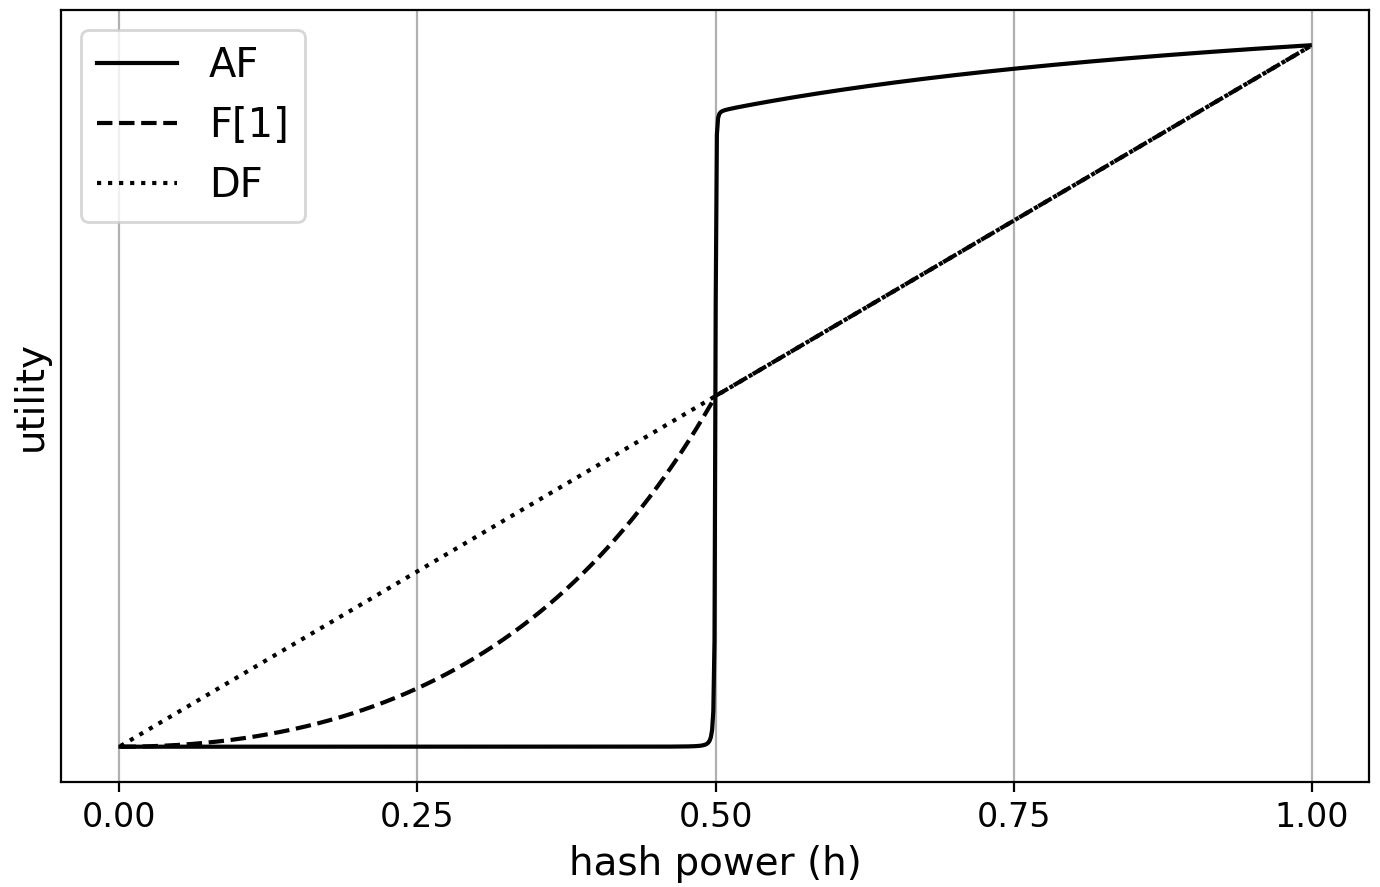
\includegraphics[width=0.46\textwidth]{plots/test_AF.png}
%    \caption{Utility for player $1$ under strategies $\bdf$, $\bpf{1}$ and $\baf$. The curve for $\bpf{1}$ is too close to that of $\df$ to tell a difference at this scale, but the difference does exist: after about $h = 0.5$, the curve for $\bpf{1}$ is always higher than that of $\df$. Note that the utility collapses to $\bdf$ when $h = 1$. This is always the highest amount that can be earned in our game.}
%        \label{fig-af-df-fo}
%\end{figure}
%
%\smallskip
%\noindent
%\francisco{I think the following subsection should not be included (or should be restated as only considering AF vs DF). The comparation with F[i] looks quite weak to me.}
%\textbf{Forking for a fixed number of times}. Looking at Figure \ref{fig-af-df-fo}, we see that the utility when using $\pf{1}$ is  between the lines for $\af$ and $\df$. 
%This utility was calculated using a similar strategy as in in the proof of Theorem \ref{thm:always_fork}. 
%From the figure one can infer that, assuming $\af$ yields more utility to player $1$ than $\df$ (e.g. when $h>0.5$), then player $1$ should not use $\pf{1}$ but rather keep on forking, as 
%the utility for $\af$ is always above than the utility for $\pf{i}$ in that case. %Can we say the same for other similar strategies? Even though we can compute the utility of using any of the strategies $\pf{i}$, we cannot directly compare an infinite number of strategies. Instead, we prove the following general result. 
%We can show something similar for all the other $\pf{i}$.
%\begin{proposition}\label{prop-fork_fix}
%Assume that $u_1(\bdf) \leq u_1(\baf)$ for some $\alpha,\beta,h$. Then for all $i > 0$ we have that $u_1((\df_0,\pf{i})) \leq u_1(\af))$.
%\end{proposition}
%
%Note that this result does not rule out the possibility that, for some amount of hash power, playing some $\pf{i}$ would turn out better than $\df$, but $\af$ would not. We know 
%this is not the case for $i = 1$, and we can also prove it for $i > 1$, albeit at the cost of much more powerful machinery that we do not have the space to introduce. 
%However, in the following section we do show that there are actually strategies leading to forks with less hash power. 

\subsection{Giving up for more utility}
\label{sec-giving-up}

%By adding a little more flexibility to the strategy of always forking, we can identify approaches that make a fork profitable with less hash power. The families of strategies that we study in this section involve two parameters. First, a \textit{give-up} parameter $\ell$ that mandates the maximum length of the fight the miner is willing to carry out when doing a fork, and a parameter $k$ that regulates how far back the miner is willing to do a fork, when confronted with a chain of blocks she does not own. We denote these strategies by $\gup_\ell^k$. 

By adding a little more flexibility to the strategy of always forking, we can identify approaches that make a fork profitable with less hash power. The families of strategies that we study in this section involve two parameters. The first parameter, denoted by $k$, regulates how far back the miner will do a fork, when confronted with a chain of blocks she does not own. The second parameter, called the \textit{give-up} time, and denoted by $\ell$, tells us the maximum number of blocks that the player's opponent is allowed to extend the current blockchain with before the player gives up mining on the forking branch. If the player does not manage to transform her fork into the new blockchain before her opponent mines $\ell$ blocks, she will restart the strategy treating the tail of the current blockchain as the new genesis block. We denote these strategies by $\gup_\ell^k$. 


\begin{figure}
\begin{center}
\begin{tikzpicture}[->,>=stealth',auto,thick, scale = 0.61,state/.style={circle,inner sep=2pt}]

    % The graph
	\node [state] at (-10.5,0) (aR) {$\varepsilon$};
	\node [state] at (-9,0) (a0) {$0$};
	\node [state] at (-7.5,0) (a00) {$00$};
	\node [state] at (-6,0) (a000) {$000$};
	\node [state] at (-9,-1.4) (aAF) {$\af$};
	\node [state] at (-7.5,-1.4) (aG) {$\gup_4^2$};
	\node [state] at (-12,-0.70) {(a)};

	% Graph edges
	\path[->]
	(aR) edge (a0)
	(a0) edge (a00)
	(a00) edge (a000);
  	
	\path[->,dashed]
	(aR) edge (aAF)
	(a0) edge (aG);
	
    % The graph
	\node [state] at (-10.5,-2.8) (bR) {$\varepsilon$};
	\node [state] at (-9,-2.8) (b0) {$0$};
	\node [state] at (-7.5,-2.8) (b00) {$00$};
	\node [state] at (-6,-2.8) (b000) {$000$};
	\node [state] at (-4,-2.8) (b0000) {$0000$};
	\node [state] at (-9,-4.3) (b1) {$1$};
	\node [state] at (-7.5,-4.3) (b11) {$11$};
	\node [state] at (-5.5,-4.3) (bAF) {$\af$};
	\node [state] at (-1.5,-2.8) (bG) {$\gup_4^2$};
	\node [state] at (-12,-3.70) {(b)};

	% Graph edges
	\path[->]
	(bR) edge (b0)
	(bR) edge (b1)
	(b1) edge (b11)
	(b0) edge (b00)
	(b00) edge (b000)
	(b000) edge (b0000);
  	
	\path[->,dashed]
	(b11) edge (bAF)
	(b0000) edge (bG);
	

\end{tikzpicture} 
\end{center}

\caption{Difference between $\af$ and $\gup^2_4$ in terms of actions of these strategies in two states. 
%In (a), the value $k = 2$ indicates that $\gup^2_4$ will not 
%fork on $\varepsilon$ but instead in $0$. In (b), the value $\ell = 4$ indicates that in this state player $1$ should give up the fork and continue mining upon the blockchain (block $0000$).
\label{fig-gup}}
\end{figure}

\begin{example}
Let us consider how $\gup_4^2$ would be different from $\af$. Since $k = 2$, both strategies take the same action when the state is $\{\varepsilon\}, \{\varepsilon,0\}$, and $\{\varepsilon,0,00\}$, namely, mining at $\varepsilon$. Hence, assume that both strategies are facing a chain of three 
%unowned new 
blocks owned by player 0, 
%in the blockchain, 
as shown in Figure \ref{fig-gup} (a). In this case, $\af$ would again try to do a fork from the genesis block as no block belongs to player 1. On the other hand, $\gup_4^2$ would try to do a fork instead on the dotted line, that is, the second block that does not belong to her.
The second difference is provided by the give-up time, which is shown in Figure~\ref{fig-gup}~(b). Normally, $\af$ is willing to continue forking regardless of the hope of winning, therefore the move for the state in Figure \ref{fig-gup} (b) would still be to mine upon her own block $11$. On the other hand, $\gup_4^2$ has already seen 4 blocks from the start of the fork, so with this strategy player $1$ instead gives up and tries to mine upon $0000$, rebooting the strategy as if 
%this last block 
$0000$ was the genesis block. Note that in fact $\af=\gup_\infty^\infty$, that is, the strategy where player $1$ is willing to keep fighting for a fork of any length, and to do a fork at the beginning of any chain of blocks she does not own.  
\end{example}

Define $\bgup_\ell^k$ as the combined strategy $(\df_0, \gup_\ell^k)$. 
To compute an analytical form for $u_1(\bgup_\ell^k)$, we proceed as in the proof of Theorem \ref{thm:always_fork}. In this case, the set of paths leading to winning states has a more complex combinatorial nature, as expected when taking into account the 
%disadvantage and give-up 
parameters $k$ and $\ell$. We obtain the following.
\begin{theorem}
For every pair of positive integers $\ell, k$ such that $k< \ell$, we have that:
$$u_1(\bgup^k_\ell) = \frac{\Phi_{\ell,k}}{1-\Gamma_{\ell,k}},$$
where $\Phi_{\ell,k}$ and $\Gamma_{\ell,k}$ are rational functions of $\alpha$, $\beta$ and $h$ (that is, divisions of polynomials of  $\alpha$, $\beta$ and $h$).
\end{theorem}
%\francisco{optional: We develop precise expressions for $\Phi_{\ell, k},\Gamma_{\ell,k}$ in appendix \ref{sec-evaluation-G}.} 
In other words, given specific values of $k$ and $\ell$, we can still compute the utility of these strategies. We use this theorem to analyse these strategies, plotting them, as we did before, 
for $\alpha = 0.9999966993$ and $\beta = 0.9999996156$. Figure \ref{fig-plot-gup-fixwindow} gives 
%us an 
interesting 
%feel 
information about the advantages of this family of strategies. 
We fix $k = 1$, plot the utility of strategies $\bgup^1_2$ through $\bgup^1_5$, and shade those areas in which one of the utilities is greater. As we see, for a 
fork window $k = 1$, the optimal amount time player $1$ should be willing to fight for a branch before giving up depends on the hash power. With little hash power the likelihood of winning a 
branch is small, so player 1 should give up as early as possible. However, the more hash power she obtains, the better it is to wait more. Interestingly, with a little more than 
$46\%$ of the hash power, player $1$ already should start using strategy $\gup^1_4$ to defeat the default strategy, and with a little more power, $\gup^1_5$. We know that player~$1$ should use $\af$ not before 
$h = 0.499$, so this gives us a lot of extra room to look for optimal strategies if we are willing to fork (especially considering that every percentage of hash power in popular cryptocurrencies 
may cost millions).

Plots for strategies with $k > 1$ present a similar behaviour: the more hash power we have, the more we should be willing to fight for our forks. However, 
Figure \ref{fig-plot-gup-fixwindow} is important because we have found that strategy $\gup^1_4$ is the strategy that beats the default strategy under the least amount of hash power 
amongst any combination of values for $k$ and $\ell$. The comparison is much less straightforward when looking at varying values of both $k$ and $\ell$, but in general, 
the more hash power the bigger the window of blocks one should aim to do a fork, and the more time one should wait before giving up. We remark that the analysis 
we can do through 2- or 3-dimensional plots is only one part of the picture, and that a game-theoretical analysis of these strategies is an interesting area for future work. 


%%%%%%%%%%%%%%%%%%%%%%%%%%%%%%%%%%%%%%%%%%%%%%%%%%%%%%%%%%%%%%%%%%%%%%%%%
%%% BELOW IS THE PREVIOUS VERSION THAT I STILL DID NOT MAKE A PASS ON %%%
%%%%%%%%%%%%%%%%%%%%%%%%%%%%%%%%%%%%%%%%%%%%%%%%%%%%%%%%%%%%%%%%%%%%%%%%%

\begin{comment}

\paragraph{Forking in the genesis block.}
The first forking strategy we models the case when 0 has won the ultimate block. The question 1 wants to answer in this situation is whether she should continue mining on the blockchain, playing according to $\df$, or should she fork, mining instead upon her previously won block? Since by the proof of Theorem \ref{thm-conts_equlibria} we know that optimal strategies for 1 depend only on the blocks following her last block in each state, we can focus on this question when the game is just starting, that is, when 1 wants to decide whether to fork in the genesis block. We will denote by $\fg_1$ the strategy in which player 1 is trying to win the first block following genesis, and once this branch becomes the new blockchain, continues mining using the default strategy. We denote by $\fg = (\df_0,\fg_1)$ the strategy where 1 tries to win the first block in the final blockchain, and 0 mines using the default strategy. A depiction of this strategy is given in Figure \ref{fig-fork_genesis}. When player 1 uses this strategy, we can compute her utility as follows.

\begin{figure}
\begin{center}
\begin{tikzpicture}[->,>=stealth',auto,thick, scale = 1.0,state/.style={circle,inner sep=2pt}]

    % The graph
	\node [state] at (0,0) (R) {$\varepsilon$};
	\node [state] at (1.5,0.75) (1) {$1$};
	\node [state] at (1.5,-0.75) (0) {$0$};
	\node [state] at (3,-0.75) (00) {$00$};
	
	\node [state] at (3,0.75) (11) {$11$};		
	\node [state] at (4.6,0.75) (111) {$111$};
	\node [state] at (6.4,0.75) (1110) {$1110$};
			

	
	% Graph edges
	\path[->]
	(R) edge (1)
	(R) edge (0)
	(0) edge (00)
	;  	
	
	\path[->,dashed]
	(1) edge (11)
	(11) edge (111)
	(111) edge (1110)
	;


\end{tikzpicture} 
\end{center}
\caption{Following the block 00 player 1 tries to win a fork starting at $\varepsilon$. Dashed edges show the case in which she succeeds, after which both players mine on top of the new blockchain.}
\label{fig-fork_genesis}
\end{figure}

\begin{myprop}
%	\label{prop-utilityofgenesisinfinite}
	\label{prop:utility_gen_fork}
%	Suppose player 1 plays with the genesis fork strategy and player 0 follows the default strategy. 
Let $h$ be the hash power of player 1. Then
	\begin{eqnarray*}
		u_1^\infty(\fg\mid\varepsilon) =K_1\cdot \Cat(\beta^2h(1-h))+K_2\cdot \Cat(\alpha\beta^2h(1-h))
	\end{eqnarray*}
where $\Cat:x\mapsto \frac{1-\sqrt{1-4x}}{2x}$ is the generating function of Catalan numbers \cite{ADD_CITATION}, and 
	\begin{eqnarray*}
		K_1 =\frac{\alpha\beta h}{(1-\alpha)(1-\beta)},\quad	K_2 =\frac{\alpha^2\beta h(\alpha\beta+h\beta-h\alpha\beta-1)}{(1-\alpha)(1-\beta)(1-\alpha\beta)}.	
	\end{eqnarray*}
\end{myprop}

The intuition behind the appearance of Catalan numbers in this result is that for each fixed $n$, the number of states where two chains of length $n$ are being tied for blockchain equals the $n$th Catalan number (more precisely, they correspond to Dyck paths of length $n$). Since such states dictate when 1 will win the desired fork, and no reward can be won by 1 before this occurs (note that the two branches in this game have only $\varepsilon$ in common), they tell us what the utility of player 1 will be. Notice that since $\beta \leq 1$, and the maximum of the function $h\mapsto h(1-h)$ is $\frac{1}{4}$, for $h\in [0,1]$, the value $Cat(\beta^2h(1-h))$ is always well defined. For the sake of completion, in Appendix \ref{appendix-gen_fork}, we also show what is the utility of $\fg$ for player 1 at each step $n$ of the mining game.

\paragraph{Forking $m$ blocks from the end of the blockchain.} The second forking strategy we consider works similarly as $\fg$, but now player 1 considers forking after losing $m$ consecutive blocks, for some fixed $m$. In this case, 1 will fork $m$ blocks from the end of the current blockchain, all of these $m$ block being owned by 0. This situation is depicted in Figure \ref{fig-fork_m}. Once player 1 wins the fork, and this branch becomes the new blockchain, she will continue mining according to $\df_1$. We denote this strategy of player 1 by $\forkm{m}_1$, and denote with $\forkm{m}=(\df_0,\forkm{m}_1)$ the strategy where 1 uses $\forkm{m}_1$, and 0 plays according to the default strategy.

\begin{figure}
\begin{center}
\begin{tikzpicture}[->,>=stealth',auto,thick, scale = 1.0,state/.style={circle,inner sep=2pt}]

    % The graph
	\node [state] at (0,0) (R) {$\varepsilon$};
	\node [state] at (1.5,0) (0) {$0$};
	\node [state] at (3,0) (01) {$01$};
	\node [state] at (4.6,0) (010) {$010$};
	\node [state] at (6.4,0) (0100) {$0100$};
	
	\node [state] at (4.6,0.75) (011) {$011$};					
	
	% Graph edges
	\path[->]
	(R) edge (0)
	(0) edge (01)
	(01) edge (010)
	(010) edge (0100)	
	;  	
	
	\path[->,dashed]
	(01) edge (011)
	;


\end{tikzpicture} 
\end{center}
\caption{If playing $\forkm{2}_1$, player 1 will try to fork after losing two consecutive blocks at position 0100. Should she manage to make the dashed branch into a blockchain, both her and player 1 continue to mine on this branch using $\df$.}
\label{fig-fork_m}
\end{figure}

When computing the utility of $\forkm{m}$ starting in some state $q_0$, we take into account that player 1 is only interested whether her utility will increase in the case she decides to fork. That is, since the blocks before her fork will always have the same constant contribution to her reward in either branch, we will not count them in the utility. With this in mind, the utility of $\forkm{m}$ starting in the state $q_0$ in which 0 has the ultimate $m$ blocks in the (up to now unique) blockchain is given as follows.

\begin{myprop}\label{prop-fork_m}
	Let $h$ be the hash power of player 1. Then
	\begin{eqnarray*}
		u_1(\mfork|q_0) =\bigg(\frac{\beta h}{\alpha}\bigg)^m K_{1}\Cat(\beta^2h(1-h))^{m+1}+(\beta h)^{m}K_{2}\Cat(\alpha\beta^2h(1-h))^{m+1}
	\end{eqnarray*}
	where $\Cat$ is as in Proposition \ref{prop:utility_gen_fork}, and 

\end{myprop}

As before, Catalan numbers help us account for all states where 1 wins the fork. Of course, now player 1 is starting with a handicap of $m$ steps, so the winning states for 1 will be characterized by staircase walks that stay inside the trapezoid $\{(0,0),(m,0),(m+n,n),(0,n)\}$, for some number $n$. The proof of this proposition is given in Appendix \ref{appendix-fork_m}.

\paragraph{When to fork?} Having the utilities of the two forking strategies, we can now compare them to that of the default strategy in order to answer whether 1 should fork or not. Analysing the curves defined by the game parameters ($\alpha,\beta$ and $h$ for $\fg$, and additionally $m$ for $\forkm{m}$), it can be seen that when $h>50\%$, and $\alpha>\beta$, then it is always convenient for 1 to fork, based on the utility resulting from either $\fg$ or (irrespective of $m$) $\forkm{m}$. This confirms the intuition that the player with the majority of hash power can sway the game in her favour, but we can also see that there are several cases when it is convenient to fork even with much lower hash power. This happens in cases when $\alpha$ is significantly bigger than $\beta$, which can be explained by the fact that ???

\end{comment}
